\documentclass{standalone}
\usepackage[dvipsnames]{xcolor}
\usepackage{tikz}
\usepackage[export]{animate}
\usepackage{ifthen}
\definecolor{darkgreen}{RGB}{10,90,10}

\begin{document}
\begin{animateinline}[controls]{30}
\multiframe{15}{i=0+6}{%
\begin{tikzpicture}[x=1cm, y=1cm]
	\path (-3,-3) to (3,3); 

	\node[draw, ultra thick, circle, minimum size=2cm, inner sep=0pt, fill=Blue] at (\i+135:1.41) {};
	\node[draw, ultra thick, circle, minimum size=2cm, inner sep=0pt, fill=Green] at (\i+45:1.41) {};
	\node[draw, ultra thick, circle, minimum size=2cm, inner sep=0pt, fill=Purple] at (\i-135:1.41) {};
	\node[draw, ultra thick, circle, minimum size=2cm, inner sep=0pt, fill=Red] at (\i-45:1.41) {};
	
	\node[draw, ultra thick, circle, minimum size=2cm, inner sep=0pt, fill=Yellow] at (5,1) {};

\end{tikzpicture}}
\newframe
\multiframe{30}{i=0+3}{%
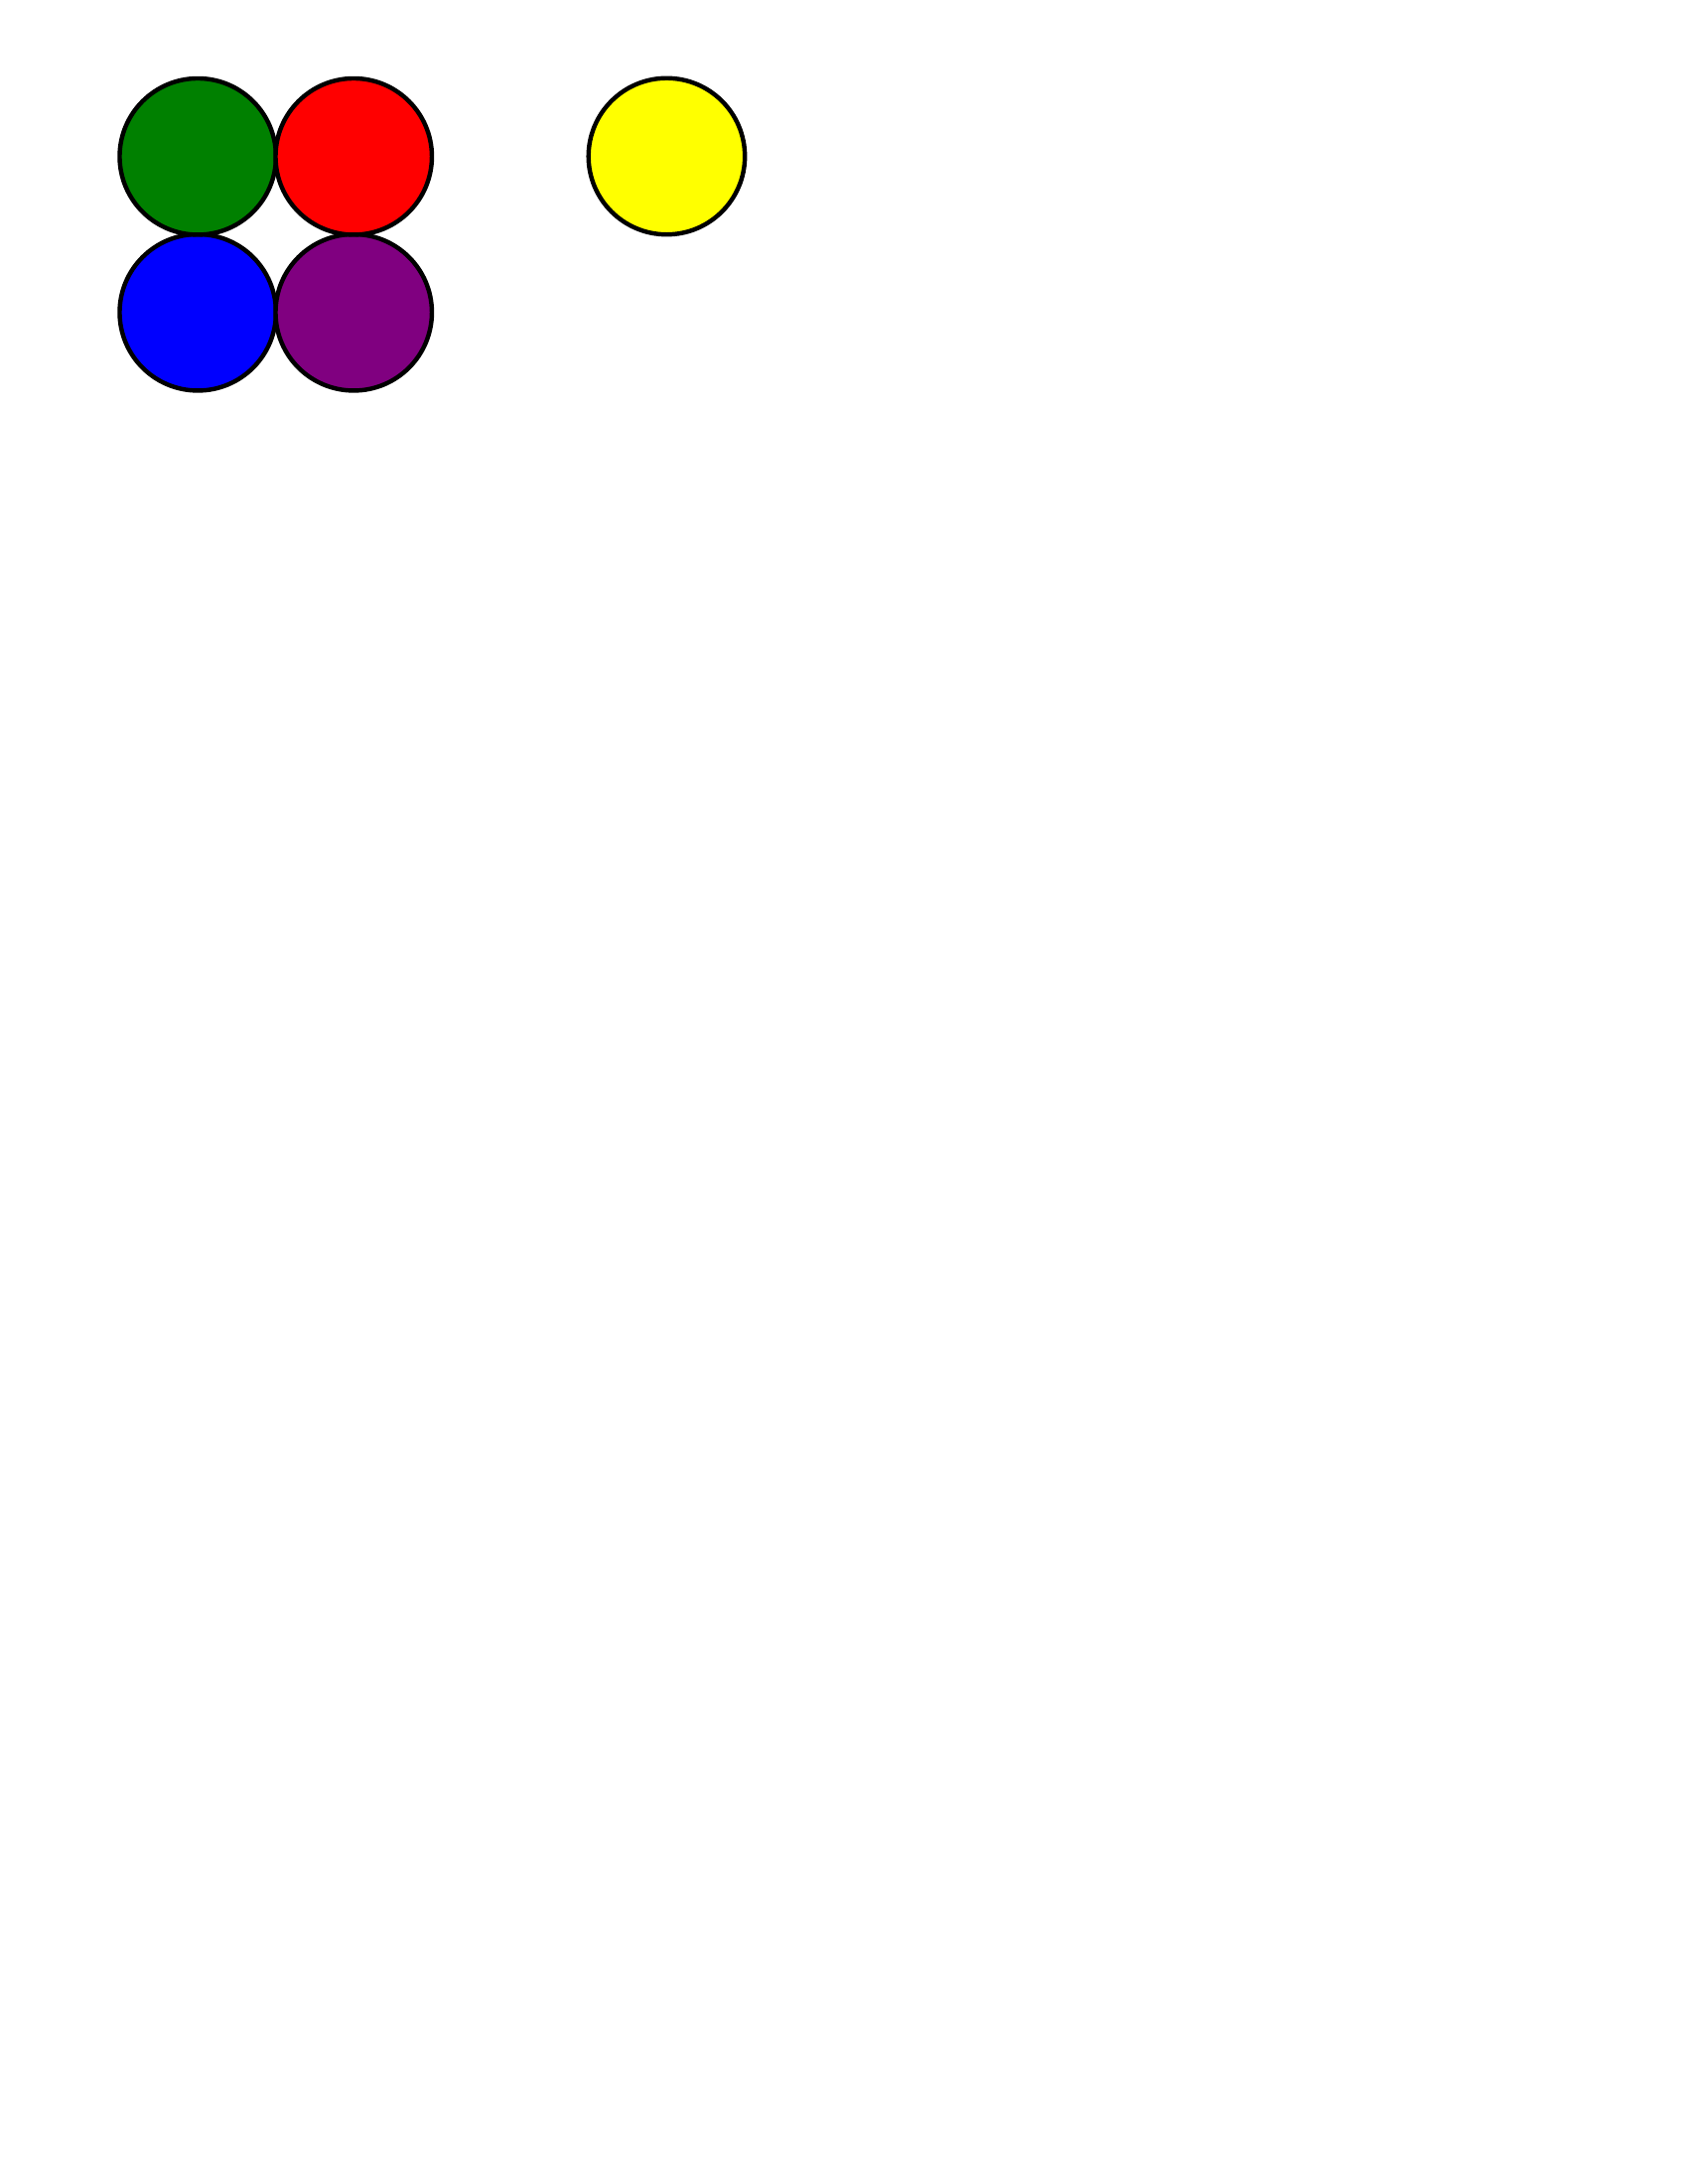
\begin{tikzpicture}[x=1cm, y=1cm]
	\path (-3,-3) to (3,3); 

	\node[draw, ultra thick, circle, minimum size=2cm, inner sep=0pt, fill=Blue] at (-135:1.41) {};
	\node[draw, ultra thick, circle, minimum size=2cm, inner sep=0pt, fill=Green] at (135:1.41) {};
	\node[draw, ultra thick, circle, minimum size=2cm, inner sep=0pt, fill=Purple] at (-45:1.41) {};
	\node[draw, ultra thick, circle, minimum size=2cm, inner sep=0pt, fill=Red] at (45:1.41) {};
	
	\node[draw, ultra thick, circle, minimum size=2cm, inner sep=0pt, fill=Yellow] at (5,1) {};
\end{tikzpicture}}
\newframe
\multiframe{15}{i=0+6}{%
\begin{tikzpicture}[x=1cm, y=1cm]
	\path (-3,-3) to (3,3); 

	\node[draw, ultra thick, circle, minimum size=2cm, inner sep=0pt, fill=Blue] at (-135+\i:1.41) {};
	\node[draw, ultra thick, circle, minimum size=2cm, inner sep=0pt, fill=Green] at (135+\i:1.41) {};
	\node[draw, ultra thick, circle, minimum size=2cm, inner sep=0pt, fill=Purple] at (-45+\i:1.41) {};
	\node[draw, ultra thick, circle, minimum size=2cm, inner sep=0pt, fill=Red] at (45+\i:1.41) {};
	
	\node[draw, ultra thick, circle, minimum size=2cm, inner sep=0pt, fill=Yellow] at (5,1) {};
\end{tikzpicture}}
\newframe
\multiframe{30}{i=0+3}{%
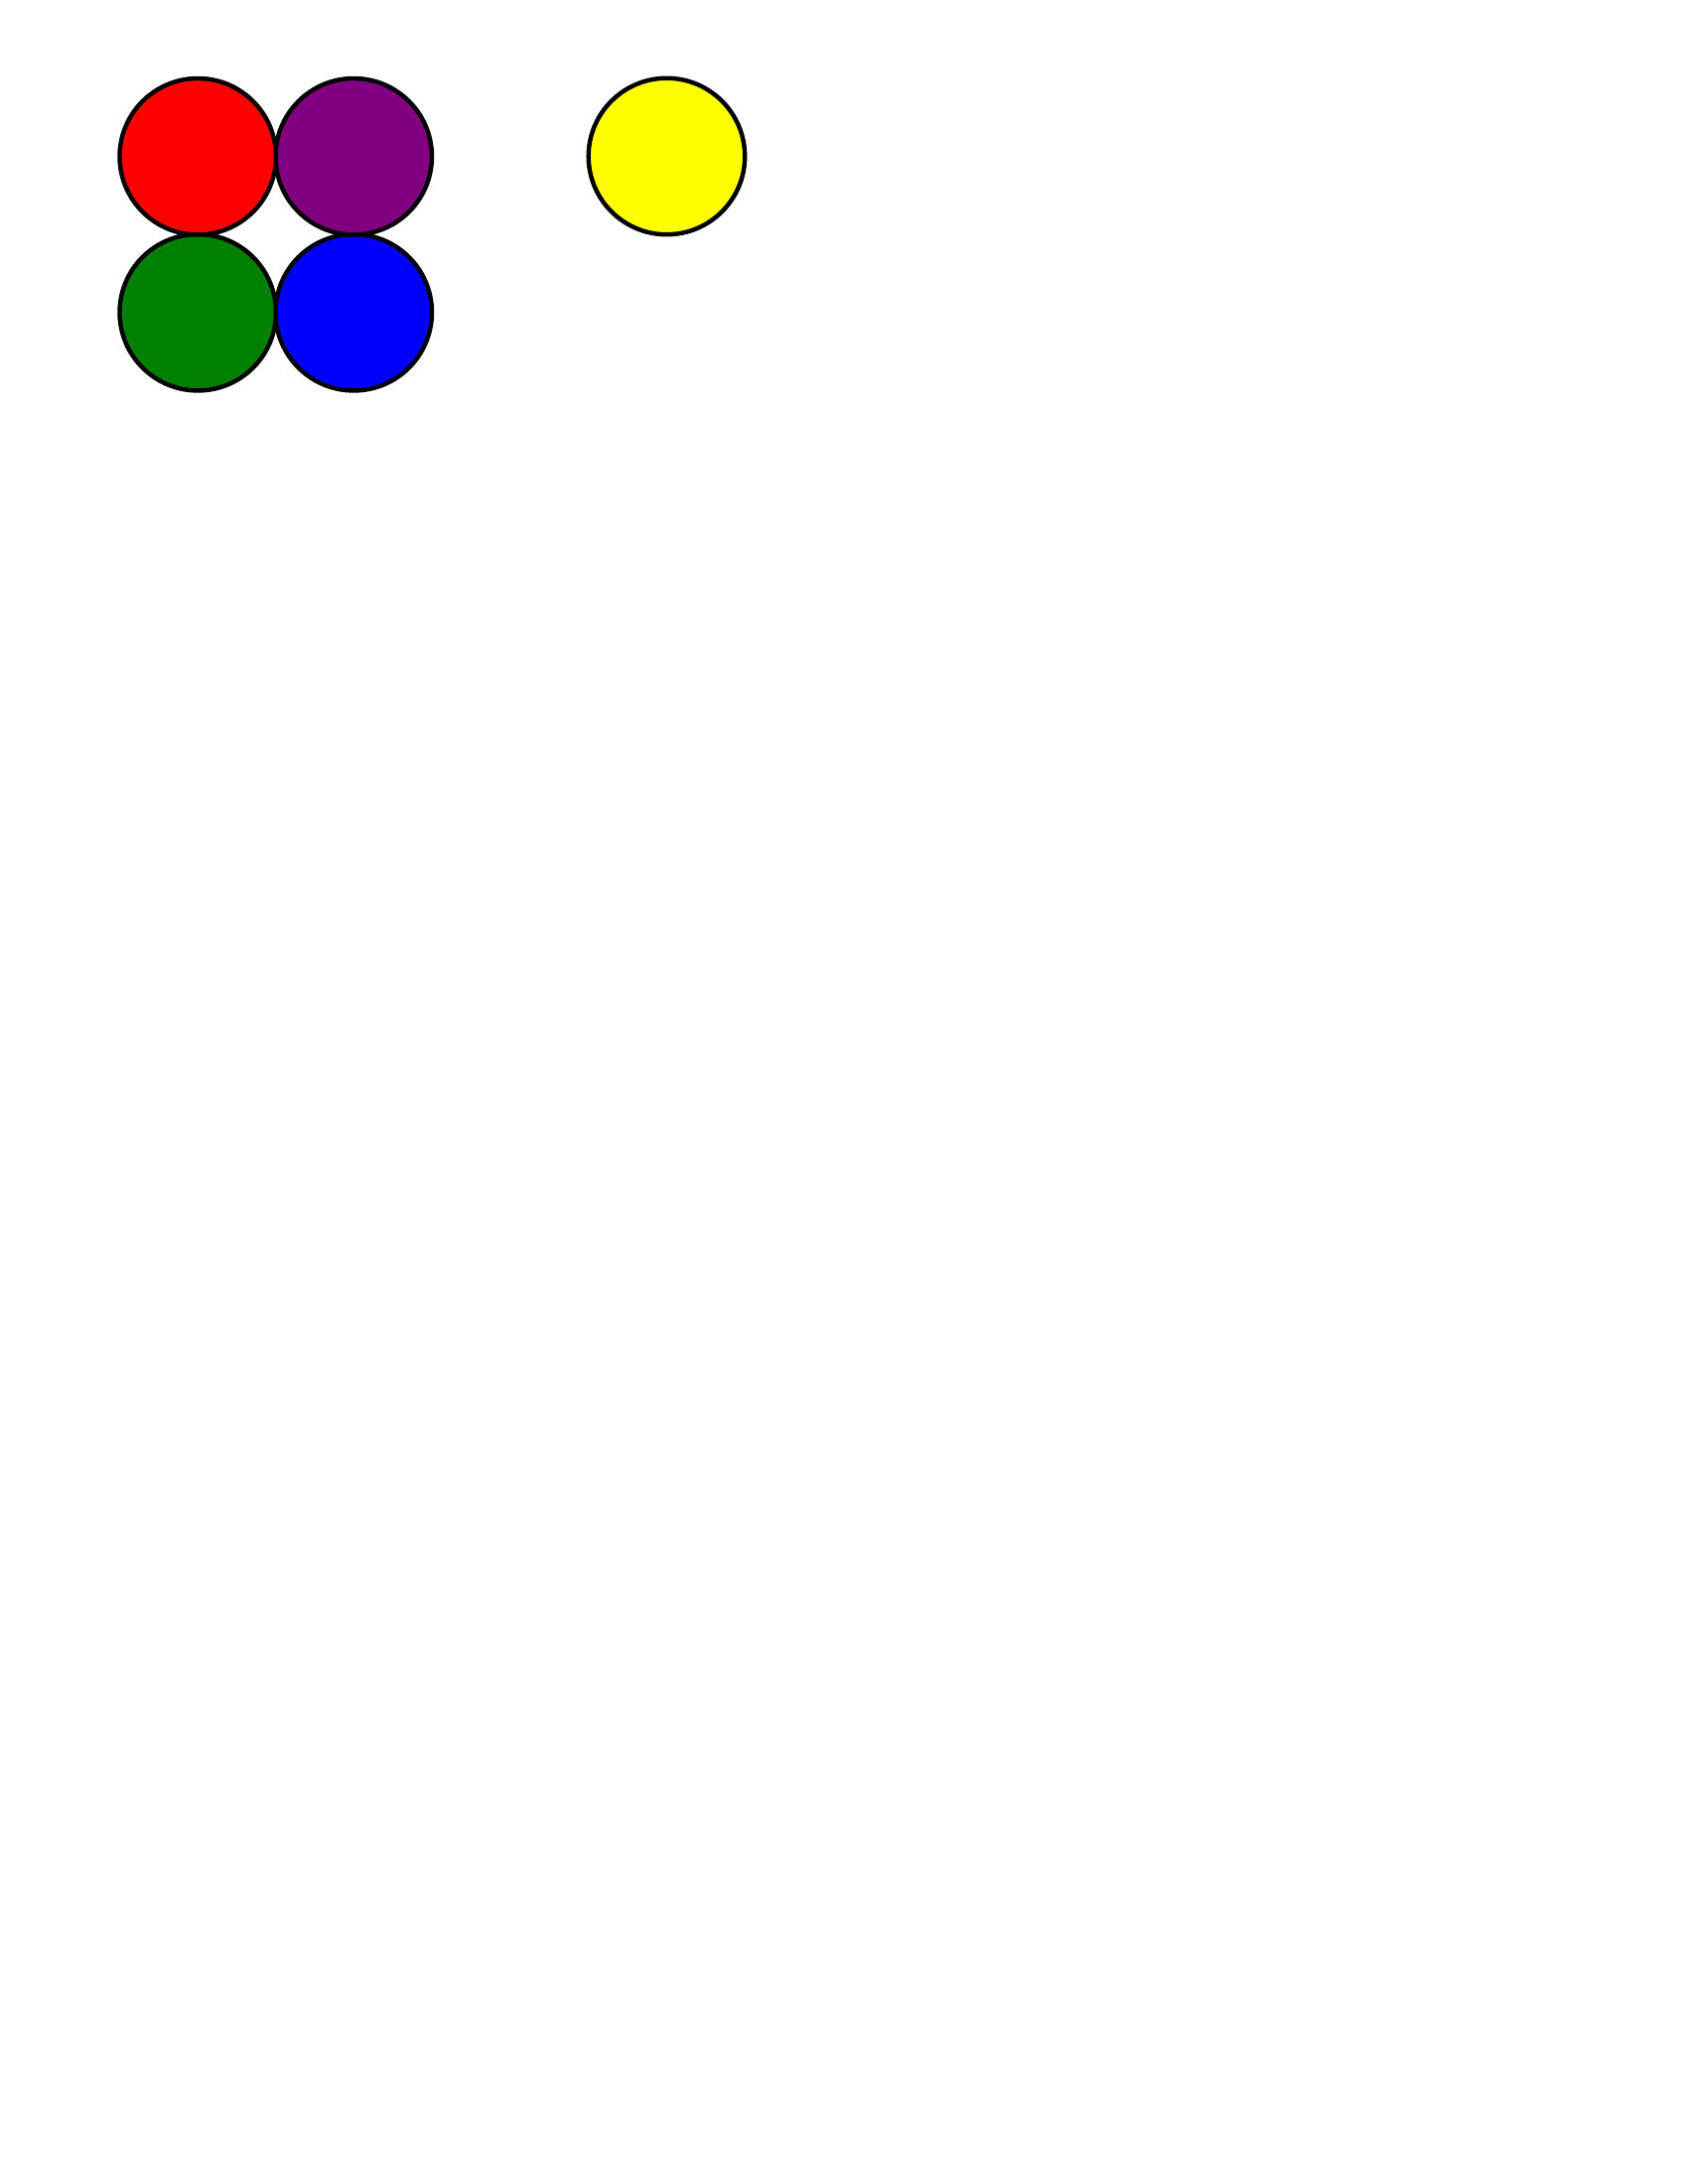
\begin{tikzpicture}[x=1cm, y=1cm]
	\path (-3,-3) to (3,3); 

	\node[draw, ultra thick, circle, minimum size=2cm, inner sep=0pt, fill=Blue] at (-45:1.41) {};
	\node[draw, ultra thick, circle, minimum size=2cm, inner sep=0pt, fill=Green] at (-135:1.41) {};
	\node[draw, ultra thick, circle, minimum size=2cm, inner sep=0pt, fill=Purple] at (45:1.41) {};
	\node[draw, ultra thick, circle, minimum size=2cm, inner sep=0pt, fill=Red] at (135:1.41) {};
	
	\node[draw, ultra thick, circle, minimum size=2cm, inner sep=0pt, fill=Yellow] at (5,1) {};
\end{tikzpicture}}
\newframe
\multiframe{15}{i=0+6}{%
\begin{tikzpicture}[x=1cm, y=1cm]
	\path (-3,-3) to (3,3); 

	\node[draw, ultra thick, circle, minimum size=2cm, inner sep=0pt, fill=Blue] at (-45+\i:1.41) {};
	\node[draw, ultra thick, circle, minimum size=2cm, inner sep=0pt, fill=Green] at (-135+\i:1.41) {};
	\node[draw, ultra thick, circle, minimum size=2cm, inner sep=0pt, fill=Purple] at (45+\i:1.41) {};
	\node[draw, ultra thick, circle, minimum size=2cm, inner sep=0pt, fill=Red] at (135+\i:1.41) {};
	
	\node[draw, ultra thick, circle, minimum size=2cm, inner sep=0pt, fill=Yellow] at (5,1) {};
\end{tikzpicture}}
\newframe
\multiframe{30}{i=0+3}{%
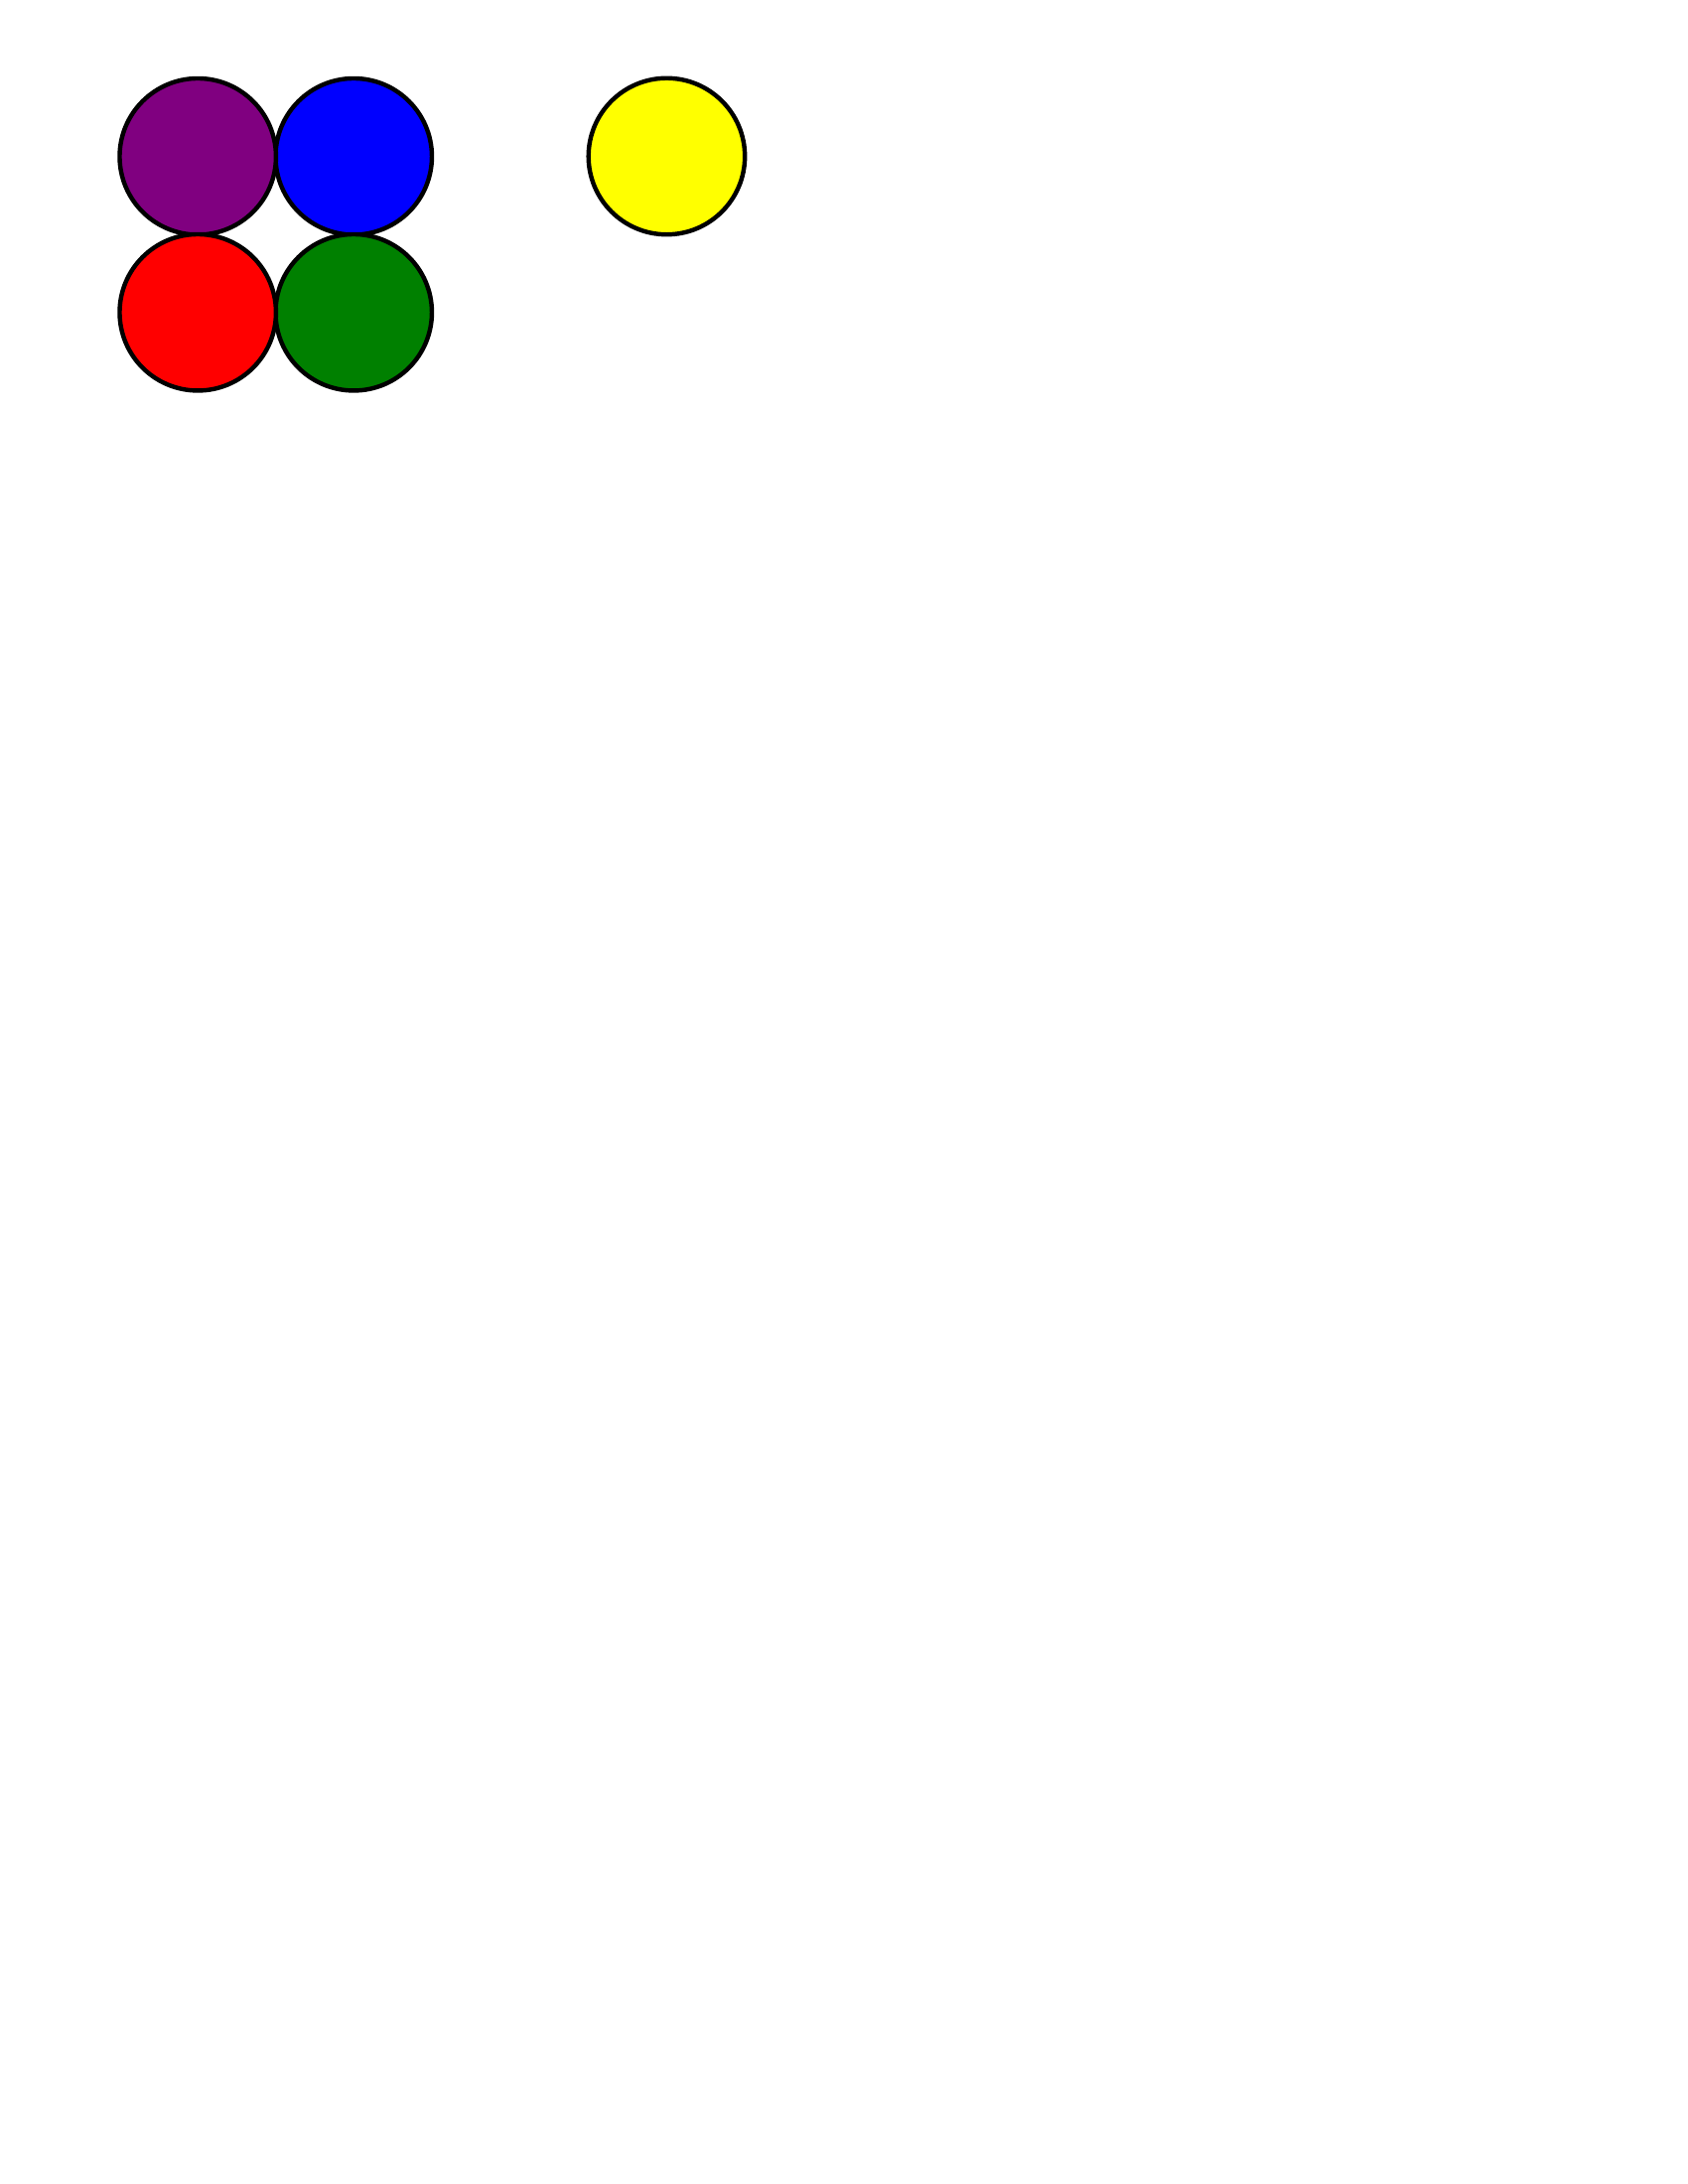
\begin{tikzpicture}[x=1cm, y=1cm]
	\path (-3,-3) to (3,3); 

	\node[draw, ultra thick, circle, minimum size=2cm, inner sep=0pt, fill=Blue] at (45:1.41) {};
	\node[draw, ultra thick, circle, minimum size=2cm, inner sep=0pt, fill=Green] at (-45:1.41) {};
	\node[draw, ultra thick, circle, minimum size=2cm, inner sep=0pt, fill=Purple] at (135:1.41) {};
	\node[draw, ultra thick, circle, minimum size=2cm, inner sep=0pt, fill=Red] at (-135:1.41) {};
	
	\node[draw, ultra thick, circle, minimum size=2cm, inner sep=0pt, fill=Yellow] at (5,1) {};
\end{tikzpicture}}
\newframe
\multiframe{15}{i=0+6}{%
\begin{tikzpicture}[x=1cm, y=1cm]
	\path (-3,-3) to (3,3); 

	\node[draw, ultra thick, circle, minimum size=2cm, inner sep=0pt, fill=Blue] at (45+\i:1.41) {};
	\node[draw, ultra thick, circle, minimum size=2cm, inner sep=0pt, fill=Green] at (-45+\i:1.41) {};
	\node[draw, ultra thick, circle, minimum size=2cm, inner sep=0pt, fill=Purple] at (135+\i:1.41) {};
	\node[draw, ultra thick, circle, minimum size=2cm, inner sep=0pt, fill=Red] at (-135+\i:1.41) {};
	
	\node[draw, ultra thick, circle, minimum size=2cm, inner sep=0pt, fill=Yellow] at (5,1) {};
\end{tikzpicture}}
\newframe
\multiframe{30}{i=0+3}{%
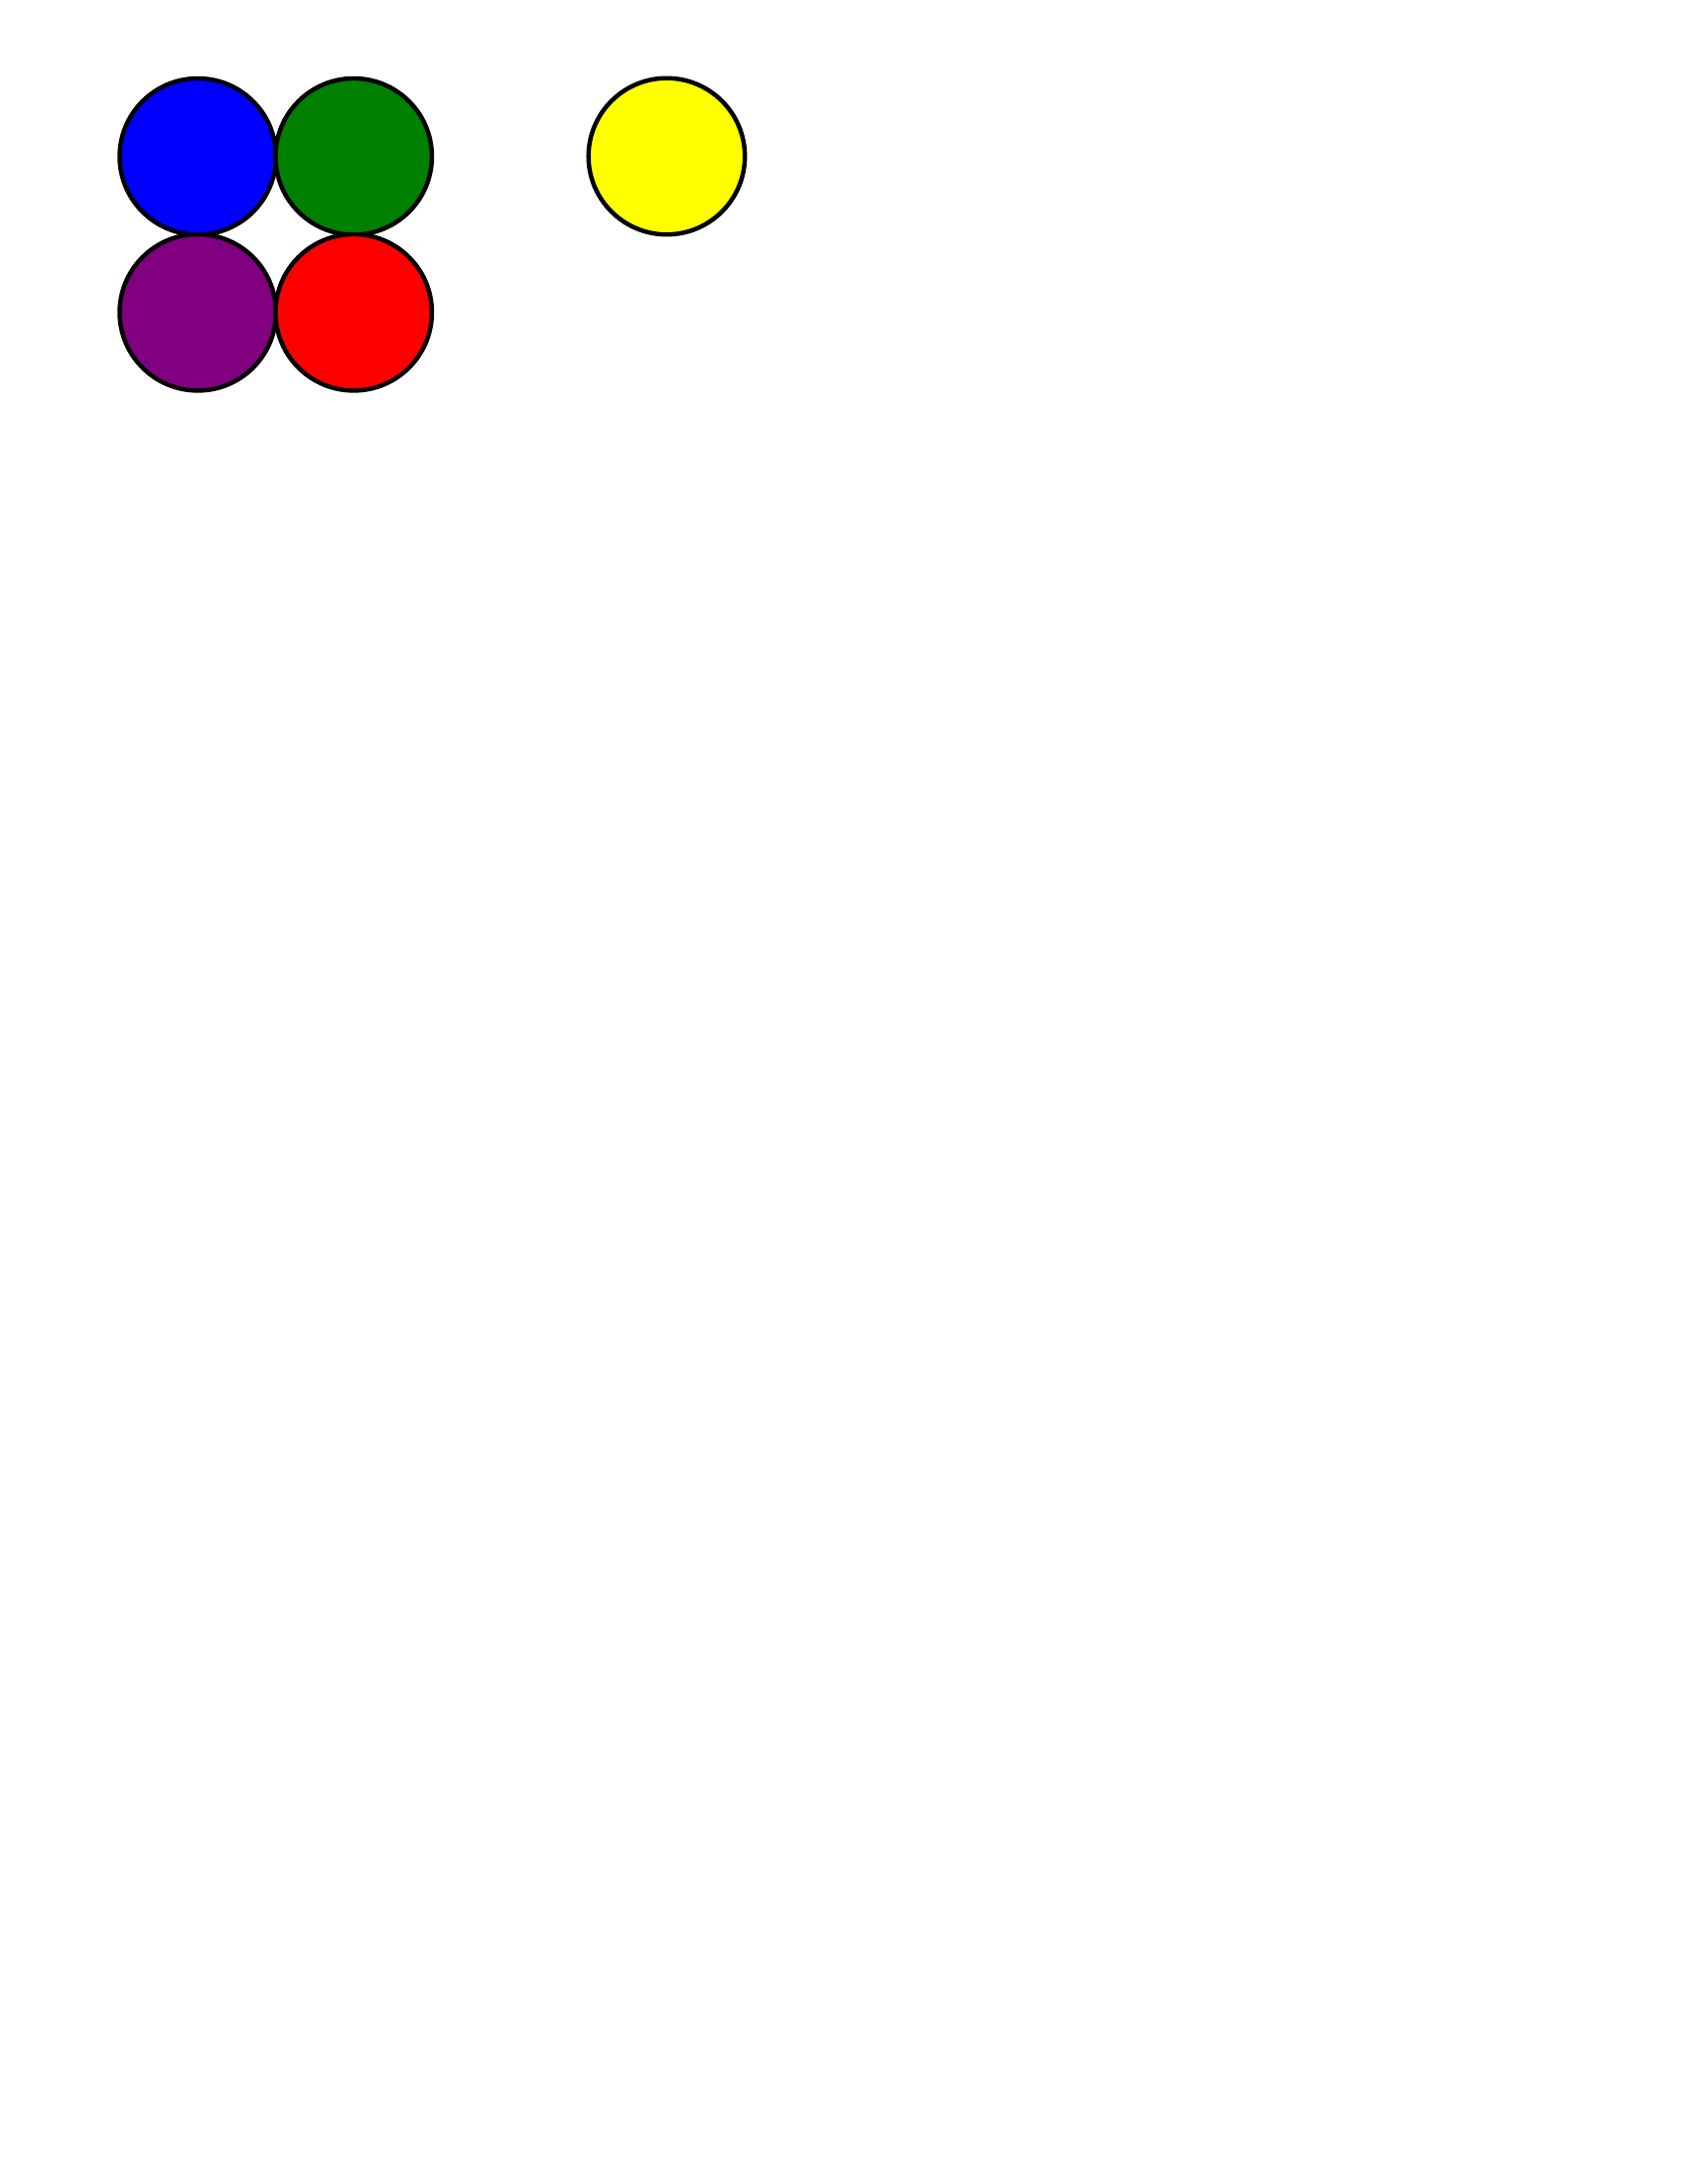
\begin{tikzpicture}[x=1cm, y=1cm]
	\path (-3,-3) to (3,3); 

	\node[draw, ultra thick, circle, minimum size=2cm, inner sep=0pt, fill=Blue] at (135:1.41) {};
	\node[draw, ultra thick, circle, minimum size=2cm, inner sep=0pt, fill=Green] at (45:1.41) {};
	\node[draw, ultra thick, circle, minimum size=2cm, inner sep=0pt, fill=Purple] at (-135:1.41) {};
	\node[draw, ultra thick, circle, minimum size=2cm, inner sep=0pt, fill=Red] at (-45:1.41) {};
	
	\node[draw, ultra thick, circle, minimum size=2cm, inner sep=0pt, fill=Yellow] at (5,1) {};

\end{tikzpicture}}

\end{animateinline}
\end{document}



